% ========= references embedded so this file is self-contained =========
\begin{filecontents*}{references.bib}
@inproceedings{He2016ResNet,
  title={Deep Residual Learning for Image Recognition},
  author={He, Kaiming and Zhang, Xiangyu and Ren, Shaoqing and Sun, Jian},
  booktitle={CVPR},
  year={2016}
}

@article{Dosovitskiy2020ViT,
  title   = {An Image is Worth 16x16 Words: Transformers for Image Recognition at Scale},
  author  = {Dosovitskiy, Alexey and Beyer, Lucas and Kolesnikov, Alexander and Weissenborn, Dirk and Zhai, Xiaohua and Unterthiner, Thomas and Dehghani, Mostafa and Minderer, Matthias and Heigold, Georg and Gelly, Sylvain and Uszkoreit, Jakob and Houlsby, Neil},
  journal = {arXiv preprint arXiv:2010.11929},
  year    = {2020}
}

@inproceedings{Lin2017FocalLoss,
  title={Focal Loss for Dense Object Detection},
  author={Lin, Tsung-Yi and Goyal, Priya and Girshick, Ross and He, Kaiming and Doll{\'a}r, Piotr},
  booktitle={ICCV},
  year={2017}
}

@misc{SpaceNetKaggle,
  title        = {SpaceNet: An Optimally Distributed Astronomy Data},
  author       = {Raza Imam},
  howpublished = {\url{https://www.kaggle.com/datasets/razaimam45/spacenet-an-optimally-distributed-astronomy-data}},
  year         = {2024},
  note         = {Accessed 2025-09-09}
}

% ---- Your Kaggle notebooks (Imbalanced SpaceNet — 40 epochs) ----
@misc{Gothi_ImbalCNN40_2025,
  author       = {Akshar Gothi},
  title        = {SpaceNet CNN (Imbalanced, 40 epochs) -- Kaggle Notebook},
  year         = {2025},
  howpublished = {\url{https://www.kaggle.com/code/akshar27/new-dataset-cnn-epoch-40}},
  note         = {Accessed 2025-09-09}
}

@misc{Gothi_ImbalViTBase40_2025,
  author       = {Akshar Gothi},
  title        = {SpaceNet ViT-Base (Imbalanced, 40 epochs) -- Kaggle Notebook},
  year         = {2025},
  howpublished = {\url{https://www.kaggle.com/code/akshar27/new-dataset-vit-epoch-40}},
  note         = {Accessed 2025-09-09}
}

% ---- Your Kaggle notebooks (Balanced SpaceNet — 40 epochs) ----
@misc{Gothi_BalEfficientNet40_2025,
  author       = {Akshar Gothi},
  title        = {Balanced SpaceNet (EfficientNetB0, 40 epochs) -- Kaggle Notebook},
  year         = {2025},
  howpublished = {\url{https://www.kaggle.com/code/akshargothi27/space-balance-efficienet}},
  note         = {Accessed 2025-09-09}
}

@misc{Gothi_BalViTBase40_2025,
  author       = {Akshar Gothi},
  title        = {Balanced SpaceNet (ViT-Base, 40 epochs) -- Kaggle Notebook},
  year         = {2025},
  howpublished = {\url{https://www.kaggle.com/code/akshargothi27/space-balance-vit-base}},
  note         = {Accessed 2025-09-09}
}

@inproceedings{EfficientNet_TanLe,
  title={EfficientNet: Rethinking Model Scaling for Convolutional Neural Networks},
  author={Tan, Mingxing and Le, Quoc},
  booktitle={ICML},
  year={2019}
}

@inproceedings{DeiT_Touvron,
  title={Training data-efficient image transformers \& distillation through attention},
  author={Touvron, Hugo and Cord, Matthieu and Douze, Matthijs and Massa, Francisco and Sablayrolles, Alexandre and J{\'e}gou, Herv{\'e}},
  booktitle={ICML},
  year={2021}
}

@misc{BiT_Kolesnikov,
  title={Big Transfer (BiT): General Visual Representation Learning},
  author={Kolesnikov, Alexander and Zhai, Xiaohua and Beyer, Lucas and others},
  year={2020},
  note={arXiv:1912.11370}
}

@inproceedings{Cui2019ClassBalanced,
  title={Class-Balanced Loss Based on Effective Number of Samples},
  author={Cui, Yin and Jia, Menglin and Lin, Tsung-Yi and Song, Yang and Belongie, Serge},
  booktitle={CVPR},
  year={2019}
}

@inproceedings{Cao2019LDAM,
  title={Learning Imbalanced Datasets with Label-Distribution-Aware Margin Loss},
  author={Cao, Kaidi and Wei, Colin and Gaidon, Adrien and Arechiga, Nuno and Ma, Tengyu},
  booktitle={NeurIPS},
  year={2019}
}

@inproceedings{Menon2021LogitAdjust,
  title={Long-tail learning via logit adjustment},
  author={Menon, Aditya Krishna and Jayasumana, Sadeep and others},
  booktitle={ICLR},
  year={2021}
}

@inproceedings{SAM_Foret,
  title={Sharpness-Aware Minimization for Efficiently Improving Generalization},
  author={Foret, Pierre and Kleiner, Ariel and Mobahi, Hossein and Neyshabur, Behnam},
  booktitle={ICLR},
  year={2021}
}
\end{filecontents*}


% ========================= main paper starts here =========================
\documentclass[conference]{IEEEtran}
\IEEEoverridecommandlockouts

\usepackage{graphicx}
\usepackage{booktabs}
\usepackage{multirow}
\usepackage{amsmath, amssymb}
\usepackage{siunitx}
\usepackage{xcolor}
\usepackage{url}
\usepackage{float}
\usepackage{placeins}
\usepackage{cite}
\usepackage{hyperref}

\newcommand{\todo}[1]{\textcolor{red}{[TODO: #1]}}

\begin{document}

\title{Convolutional Neural Nets vs Vision Transformers: A SpaceNet Case Study with Balanced vs Imbalanced Regimes}

\author{\IEEEauthorblockN{Akshar Gothi}
\IEEEauthorblockA{Department of Computer Science\\San Francisco State University\\San Francisco, CA, USA\\\texttt{akshargothi70@gmail.com}}}

\maketitle

\begin{abstract}
We present a controlled comparison of a convolutional neural network (CNN; EfficientNetB0) and Vision Transformers (ViT-Base) under two label-distribution regimes on the same dataset: SpaceNet (astronomical images). Using a naturally imbalanced five-class split and a balanced-resampled version constructed from the same images (700/class overall), we evaluate accuracy, macro-F1, balanced accuracy, per-class recall, and deployment metrics (latency, model size). Imbalanced experiments (40 epochs) show EfficientNetB0 reaching \SI{93}{\percent} test accuracy with strong macro-F1, while ViT-Base is competitive at \SI{93}{\percent} but with higher parameter count and latency. On balanced SpaceNet (40 epochs), both models are strong; EfficientNetB0 reaches \SI{99}{\percent} and ViT-Base is competitive, with the CNN retaining a size/latency edge.
\end{abstract}

\begin{IEEEkeywords}
Vision Transformer, EfficientNet, Class Imbalance, Robustness, SpaceNet, Astronomy, Image Classification
\end{IEEEkeywords}

\section{Introduction}
Convolutional neural networks (CNNs) remain the workhorse of image classification, while Vision Transformers (ViTs) have rapidly matched or surpassed CNN accuracy in many regimes~\cite{He2016ResNet,Dosovitskiy2020ViT}. Beyond raw accuracy, however, practical deployments care about (i) robustness to label \emph{imbalance}, (ii) behavior under distribution shift and noise, and (iii) efficiency (parameters, latency, and training cost). To study these factors cleanly, we hold the \emph{content} fixed and vary only the \emph{label distribution} on a single dataset, SpaceNet. Specifically, we compare CNNs (EfficientNetB0) and ViTs (Base/Small/Tiny) on: (i) a \textbf{naturally imbalanced} five-class split (\emph{asteroid, black hole, comet, nebula, constellation}; counts in Table~\ref{tab:spacenet_counts_imbal}), and (ii) a \textbf{balanced-resampled} split with exactly \textbf{700 images/class} and a \textbf{70:20:10} train–val–test directory structure (Table~\ref{tab:balanced_counts}). 

\paragraph*{Study design.}
All experiments use $224\!\times\!224$ inputs, ImageNet normalization, lightweight geometric augmentations, and identical evaluation metrics. For both regimes (imbalanced and balanced), we train \textbf{40 epochs} for \emph{EfficientNetB0} and \emph{ViT-Base}. We report accuracy, macro-F1, balanced accuracy, per-class precision/recall/F1, and deployment metrics (model size, dataset inference time, and training time) on an NVIDIA P100. All code, seeds, and predictions are available via our Kaggle notebooks~\cite{Gothi_ImbalCNN40_2025,Gothi_ImbalViTBase40_2025,Gothi_BalEfficientNet40_2025,Gothi_BalViTBase40_2025}.

\paragraph*{Preview of findings.}
On the imbalanced split, EfficientNetB0 attains strong macro-F1 with \SI{93}{\percent} test accuracy (40 epochs) and favorable latency, while ViT-Base is competitive at \SI{93}{\percent} with higher parameter count and runtime. On the balanced split, all models exceed \SI{93}{\percent} accuracy, with EfficientNetB0 reaching \SI{99}{\percent} and ViT-Tiny \SI{98}{\percent}, underscoring that class balance narrows architecture gaps while CNNs preserve an efficiency edge. These results align with cross-domain evidence suggesting ViTs may be comparatively robust (e.g., to weather noise, OOD) whereas CNNs can be more parameter/latency efficient, and sometimes more \emph{specialized}.

\paragraph*{Contributions.}
\begin{enumerate}
    \item A controlled, single-dataset comparison of \textbf{CNNs vs ViTs} under \textbf{two label distributions} (imbalanced vs balanced) with matched preprocessing, budgets, and metrics.
    \item A detailed report spanning \textbf{macro-F1, balanced accuracy, per-class recall}, plus \textbf{deployment metrics} (model size, dataset inference time, training time).
    \item \textbf{Reproducible artifacts}: we release prediction CSVs and training logs from all runs; the paper auto-includes per-class tables, confusion matrices, and learning curves via simple CSV exports.
    \item \textbf{Practical guidance}: when labels are skewed and latency matters, CNNs (EfficientNetB0) are a strong default; when classes are balanced or robustness is paramount, ViTs (or hybrids) become attractive.
\end{enumerate}


\section{Related Work}
\textbf{CNN/ViT foundations.} EfficientNet scales depth/width/resolution with compound coefficients and remains a strong accuracy–efficiency baseline among CNNs~\cite{EfficientNet_TanLe}. ViT dispenses with convolutional inductive biases and models global context via self-attention, typically benefiting from large-scale pretraining~\cite{Dosovitskiy2020ViT}. Data-efficient Image Transformers (DeiT) reduce ViT’s data hunger via distillation and regularization~\cite{DeiT_Touvron}. Big Transfer (BiT) further shows that strong pretraining substantially improves downstream performance and robustness~\cite{BiT_Kolesnikov}.

\textbf{Imbalance and long-tailed recognition.} Class imbalance degrades minority recall and macro metrics. Beyond focal loss~\cite{Lin2017FocalLoss}, common remedies include re-weighting with the \emph{effective number of samples} (Class-Balanced Loss)~\cite{Cui2019ClassBalanced}, margin-based LDAM with deferred re-weighting (LDAM-DRW)~\cite{Cao2019LDAM}, and logit-adjustment by label priors for calibrated long-tail predictions~\cite{Menon2021LogitAdjust}. Empirically, ViTs often rely more on pretraining and stronger regularization under skew, whereas well-tuned CNNs (with simple re-weighting) can be competitive at lower compute. Our SpaceNet results are consistent with this pattern.

\section{Dataset and Splits}
\subsection{SpaceNet (Kaggle)} We use the SpaceNet astronomy dataset\cite{SpaceNetKaggle}. Corrupted images (header/decoding failures) were removed prior to splitting.

\subsection{Imbalanced 5-Class Split (SpaceNet-5)}
\begin{table}[!t]
\centering
\caption{SpaceNet-5 (Imbalanced): per-class image counts by split.}
\begin{tabular}{lrrrr}
\toprule
\textbf{Class} & \textbf{Train} & \textbf{Val} & \textbf{Test} & \textbf{Total} \\
\midrule
Asteroid      & 182  & 76  & 25  & 283  \\
Black Hole    & 456  & 134 & 66  & 656  \\
Comet         & 290  & 80  & 46  & 416  \\
Nebula        & 831  & 254 & 107 & 1192 \\
Constellation & 1110 & 276 & 166 & 1552 \\
\midrule
\textbf{Total} & \textbf{2869} & \textbf{820} & \textbf{410} & \textbf{4099} \\
\bottomrule
\end{tabular}
\label{tab:spacenet_counts_imbal}
\end{table} 
\noindent\textit{Skew.} Largest-to-smallest in the train split is $\sim 6.1\times$.

\subsection{Balanced-Resampled 5-Class Split}

\paragraph{Balancing strategy (oversampling via augmentation).}
To construct the balanced split (\textbf{700 images per class}; Table~\ref{tab:balanced_counts}), we upsampled minority classes \emph{only in the training set} using on-the-fly data augmentation until each class reached \textbf{490} train images (the 70\% portion). Validation (140/class) and test (70/class) remain \emph{unaltered} to avoid leakage.

\noindent For majority classes with $n_c^{\text{train}} > T_{\text{train}}$, we perform random \emph{downsampling without replacement} to $T_{\text{train}}$. All random splits and sampling operations use a fixed seed (\texttt{seed}=42) for reproducibility.

Let $T{=}700$ and $(T_{\text{train}},T_{\text{val}},T_{\text{test}}){=}(490,140,70)$. For each class $c$ with original counts $(n_c^{\text{train}}, n_c^{\text{val}}, n_c^{\text{test}})$, we sample with replacement from the class’s \emph{train} pool and apply an augmentation operator $A(\cdot)$ until $n_c^{\text{train}}$ reaches $T_{\text{train}}$. The operator $A$ comprises lightweight, astronomy-plausible transforms:
\[
\begin{aligned}
A = \{\, & \text{rotation }(\pm 20^\circ),\ \text{horizontal flip }(p{=}0.5), \\
         & \text{translation }(\leq 10\%),\ \text{zoom }([0.9, 1.1]), \\
         & \text{shear }(\pm 10^\circ),\ \text{brightness/contrast }(\pm 10\%), \\
         & \text{Gaussian noise }(\sigma{=}0.01)\, \}.
\end{aligned}
\]

We avoid extreme color shifts or cut-paste operations to preserve astrophysical realism. All augmentations are applied \emph{only} to the training split; validation and test images are kept as originally sampled.

\begin{table}[!t]
\centering
\caption{Balanced SpaceNet-5 (700/class, 70:20:10): per-class image counts by split.}
\begin{tabular}{lrrrr}
\toprule
\textbf{Class} & \textbf{Train (70\%)} & \textbf{Val (20\%)} & \textbf{Test (10\%)} & \textbf{Total} \\
\midrule
Asteroid       & 490 & 140 & 70 & 700 \\
Black Hole     & 490 & 140 & 70 & 700 \\
Comet          & 490 & 140 & 70 & 700 \\
Nebula         & 490 & 140 & 70 & 700 \\
Constellation  & 490 & 140 & 70 & 700 \\
\midrule
\textbf{Total} & \textbf{2450} & \textbf{700} & \textbf{350} & \textbf{3500} \\
\bottomrule
\end{tabular}
\label{tab:balanced_counts}
\end{table}

\section{Models and Training}

\paragraph*{Architectures.}
We evaluate a lightweight CNN and three ViT variants:
\emph{EfficientNetB0} ($\sim$4.06M params) and \emph{ViT-Base/Small/Tiny} ($\sim$85.8M / 21.7M / 5.53M params).
ViT models use patch size $16\times16$ (vit-*-patch16-224) with a class token and linear head.

\begin{table}[!t]
\centering
\caption{Architectural summary used in our runs (40 epochs).}
\begin{tabular}{lrrrr}
\toprule
Model          & Params & Patch & DropPath & Head Drop \\
\midrule
EfficientNetB0 & 4.06M  & --    & --       & 0.1 \\
ViT-Base       & 85.8M  & 16    & 0.10     & 0.1 \\
ViT-Small      & 21.7M  & 16    & 0.10     & 0.1 \\
ViT-Tiny       & 5.53M  & 16    & 0.10     & 0.1 \\
\bottomrule
\end{tabular}
\label{tab:model_configs}
\end{table}


\paragraph*{Preprocessing \& Augmentation.}
All images are resized to $224\times224$ and normalized with ImageNet statistics.
Train-time augmentations follow our Kaggle code: rescale, rotation, shift, shear, zoom, and horizontal flip.
Eval-time uses a direct resize to $224\times224$ (no crop).

\paragraph*{Optimization.}
CNNs use Adam ($\mathrm{lr}{=}10^{-4}$, $\beta{=}(0.9,0.999)$). ViTs use AdamW ($\mathrm{lr}{=}10^{-4}$, $\beta{=}(0.9,0.999)$) with weight decay $10^{-2}$ (bias and LayerNorm excluded).
Batch size is 16. Unless otherwise stated, the learning rate is constant (no scheduler).
Training is in mixed precision on a single NVIDIA P100.

\paragraph*{Regimes \& Epoch Budgets.}
\textbf{Imbalanced} SpaceNet-5: EfficientNetB0 and ViT-Base trained for \textbf{40 epochs}.
\textbf{Balanced} SpaceNet-5: EfficientNetB0 and ViT-Base trained for \textbf{40 epochs}.
(Exact split sizes are in Tables~\ref{tab:spacenet_counts_imbal} and \ref{tab:balanced_counts}.)

\subsection{Imbalance Handling}
We consider three standard objectives on the imbalanced split:
(i) uniform cross-entropy; (ii) \textbf{class-weighted} cross-entropy with
$w_c=\frac{N}{K\,n_c}$ yielding weights: asteroid 3.153, black hole 1.258, comet 1.979, nebula 0.690, constellation 0.517; and
(iii) \textbf{focal loss} with focusing parameter $\gamma\in\{1,2\}$~\cite{Lin2017FocalLoss}.
Unless noted, sampling remains uniform (no class-balanced sampler).

\section{Metrics \& Protocol}

\paragraph*{Primary metrics.}
We report \textbf{Accuracy}, \textbf{Macro-F1} (unweighted class average), and \textbf{Balanced Accuracy} ($\frac{1}{K}\sum_{c}\mathrm{TPR}_c$).
We also include \textbf{per-class} Precision/Recall/F1 and confusion matrices in the main text or appendix.

\paragraph*{Uncertainty.}
For Macro-F1 and per-class Recall we compute \textbf{95\% bootstrap confidence intervals} using 10{,}000 resamples of the test set (with replacement).

\paragraph*{Latency \& efficiency.}
We measure \emph{dataset inference time} (wall clock) on the full test set and convert to \emph{ms/img} as a deployment proxy. Per-image latency uses batch size 1; dataset time uses the full test loader. Each metric is averaged over 5 runs after 100 warmup iterations. We also report \emph{model size} (MB). All runs use the same P100 GPU.

\section{Results}
\subsection{Imbalanced SpaceNet-5 (40 epochs)}
Summary of your consolidated runs:

\begin{table}[!t]
\centering
\caption{Imbalanced SpaceNet-5 (5 classes). Test metrics at 40 epochs (P100).}
\begin{tabular}{lcccc}
\toprule
\textbf{Model (40 ep)} & Acc & Prec & Rec & F1 \\
\midrule
EfficientNetB0 & 0.92 & 0.93 & 0.93 & 0.93 \\
ViT-Base       & 0.93 & 0.92 & 0.92 & 0.92 \\
\bottomrule
\end{tabular}
\label{tab:imbal_main}
\end{table}

\noindent\textbf{Efficiency.} Dataset inference time (s): EffB0 (60.3), ViT-Base (76.3), ViT-Small (75.0), ViT-Tiny (77.3). Model sizes (MB): 46.97 / 327.31 / 82.66 / 21.08. Training time per epoch (s): 231.7 / 747.8 / 710.8 / 723.9.

\subsection{Balanced SpaceNet-5 (40 epochs)}
All models are strong; CNN is most accurate and fastest overall.

\begin{table}[!t]
\centering
\caption{Balanced SpaceNet-5 (5 classes, 700/class overall). Test metrics at 40 epochs.}
\begin{tabular}{lcccc}
\toprule
\textbf{Model (40 ep)} & Acc & Prec & Rec & F1 \\
\midrule
EfficientNetB0 & 0.99 & 0.99 & 0.99 & 0.99 \\
ViT-Base       & 0.93 & 0.97 & 0.97 & 0.97 \\
\bottomrule
\end{tabular}
\label{tab:bal_main}
\end{table}

% --- Keep the tables here so they don't float away ---
\subsection{Imbalanced SpaceNet-5 (40 epochs)}
\label{sec:imbal_results_40}

\FloatBarrier  % flush anything above; start clean here

\begin{table}[!t]
\centering
\caption{Imbalanced SpaceNet-5 — CNN (EfficientNetB0). Selected epochs.}
\label{tab:imbal_cnn_subset}
\begin{tabular}{r
S[table-format=1.4]
S[table-format=1.4]
S[table-format=1.4]
S[table-format=1.4]}
\toprule
\textbf{Epoch} & \textbf{Train Loss} & \textbf{Val Loss} & \textbf{Train Acc} & \textbf{Val Acc} \\
\midrule
 1  & 1.0918 & 1.8562 & 0.6481 & 0.1066 \\
 5  & 0.4216 & 0.7094 & 0.8882 & 0.7806 \\
10  & 0.1759 & 0.8635 & 1.0000 & 0.5000 \\
15  & 0.2417 & 0.3845 & 0.9372 & 0.9142 \\
20  & 0.1627 & 0.3063 & 1.0000 & 1.0000 \\
30  & 0.0815 & 0.0649 & 1.0000 & 1.0000 \\
40  & 0.0895 & 1.0819 & 1.0000 & 0.5000 \\
\bottomrule
\end{tabular}
\end{table}

\begin{table}[!t]
\centering
\caption{Imbalanced SpaceNet-5 — ViT-Base. Selected epochs (rounded).}
\label{tab:imbal_vit_subset}
\begin{tabular}{r
S[table-format=1.3]
S[table-format=1.3]
S[table-format=1.3]
S[table-format=1.3]
S[table-format=1.3]
S[table-format=1.3]}
\toprule
\textbf{Epoch} & \textbf{Train Loss} & \textbf{Val Loss} & \textbf{Acc} & \textbf{F1} & \textbf{Prec} & \textbf{Rec} \\
\midrule
 1  & 0.295 & 0.344 & 0.873 & 0.873 & 0.879 & 0.873 \\
 5  & 0.088 & 0.296 & 0.899 & 0.898 & 0.900 & 0.899 \\
10  & 0.026 & 0.360 & 0.908 & 0.908 & 0.909 & 0.908 \\
15  & 0.011 & 0.435 & 0.914 & 0.914 & 0.916 & 0.914 \\
20  & 0.004 & 0.467 & 0.918 & 0.918 & 0.920 & 0.918 \\
30  & 0.012 & 0.535 & 0.913 & 0.913 & 0.915 & 0.913 \\
40  & 0.022 & 0.578 & 0.913 & 0.913 & 0.915 & 0.913 \\
\bottomrule
\end{tabular}
\end{table}

\FloatBarrier  % keep these two together before continuing

\subsection{Balanced SpaceNet-5 (40 epochs)}
\label{sec:bal_results_40}

\FloatBarrier 

We summarize selected-epoch training and validation statistics for both models in
Tables~\ref{tab:bal_cnn_subset} and \ref{tab:bal_vit_subset}. These follow the same
metric definitions and evaluation protocol described in Section~V.

\begin{table}[!t]
\centering
\caption{Balanced SpaceNet-5 — CNN (EfficientNetB0). Selected epochs.}
\label{tab:bal_cnn_subset}
\begin{tabular}{r
S[table-format=1.4]
S[table-format=1.4]
S[table-format=1.4]
S[table-format=1.4]}
\toprule
\textbf{Epoch} & \textbf{Train Loss} & \textbf{Val Loss} & \textbf{Train Acc} & \textbf{Val Acc} \\
\midrule
 1  & 1.0402 & 1.9168 & 0.6859 & 0.1890 \\
 5  & 0.3133 & 1.3532 & 0.9297 & 0.5683 \\
10  & 0.1416 & 0.3880 & 1.0000 & 0.9167 \\
15  & 0.1454 & 0.2189 & 0.9781 & 0.9782 \\
20  & 0.1289 & 0.0938 & 1.0000 & 1.0000 \\
30  & 0.0932 & 0.0622 & 1.0000 & 1.0000 \\
40  & 0.0877 & 0.0623 & 1.0000 & 1.0000 \\
\bottomrule
\end{tabular}
\end{table}

\begin{table}[!t]
\centering
\caption{Balanced SpaceNet-5 — ViT-Base. Selected epochs (rounded).}
\label{tab:bal_vit_subset}
\begin{tabular}{r
S[table-format=1.3]
S[table-format=1.3]
S[table-format=1.3]
S[table-format=1.3]
S[table-format=1.3]
S[table-format=1.3]}
\toprule
\textbf{Epoch} & \textbf{Train Loss} & \textbf{Val Loss} & \textbf{Acc} & \textbf{F1} & \textbf{Prec} & \textbf{Rec} \\
\midrule
 1  & 0.207 & 0.166 & 0.960 & 0.960 & 0.961 & 0.960 \\
 5  & 0.017 & 0.207 & 0.954 & 0.955 & 0.958 & 0.954 \\
10  & 0.000 & 0.101 & 0.976 & 0.976 & 0.976 & 0.976 \\
15  & 0.010 & 0.170 & 0.970 & 0.970 & 0.971 & 0.970 \\
20  & 0.000 & 0.186 & 0.967 & 0.967 & 0.968 & 0.967 \\
30  & 0.000 & 0.194 & 0.969 & 0.969 & 0.969 & 0.969 \\
40  & 0.000 & 0.198 & 0.970 & 0.970 & 0.970 & 0.970 \\
\bottomrule
\end{tabular}
\end{table}

\FloatBarrier  % ensure all four tables stay before the next figures/text

% --- Row 1 (Balanced) ---
\subsection{Confusion matrices}
\begin{figure*}[!t]
\centering

% Row 1 (Balanced)
\begin{minipage}{0.48\textwidth}
  \centering
  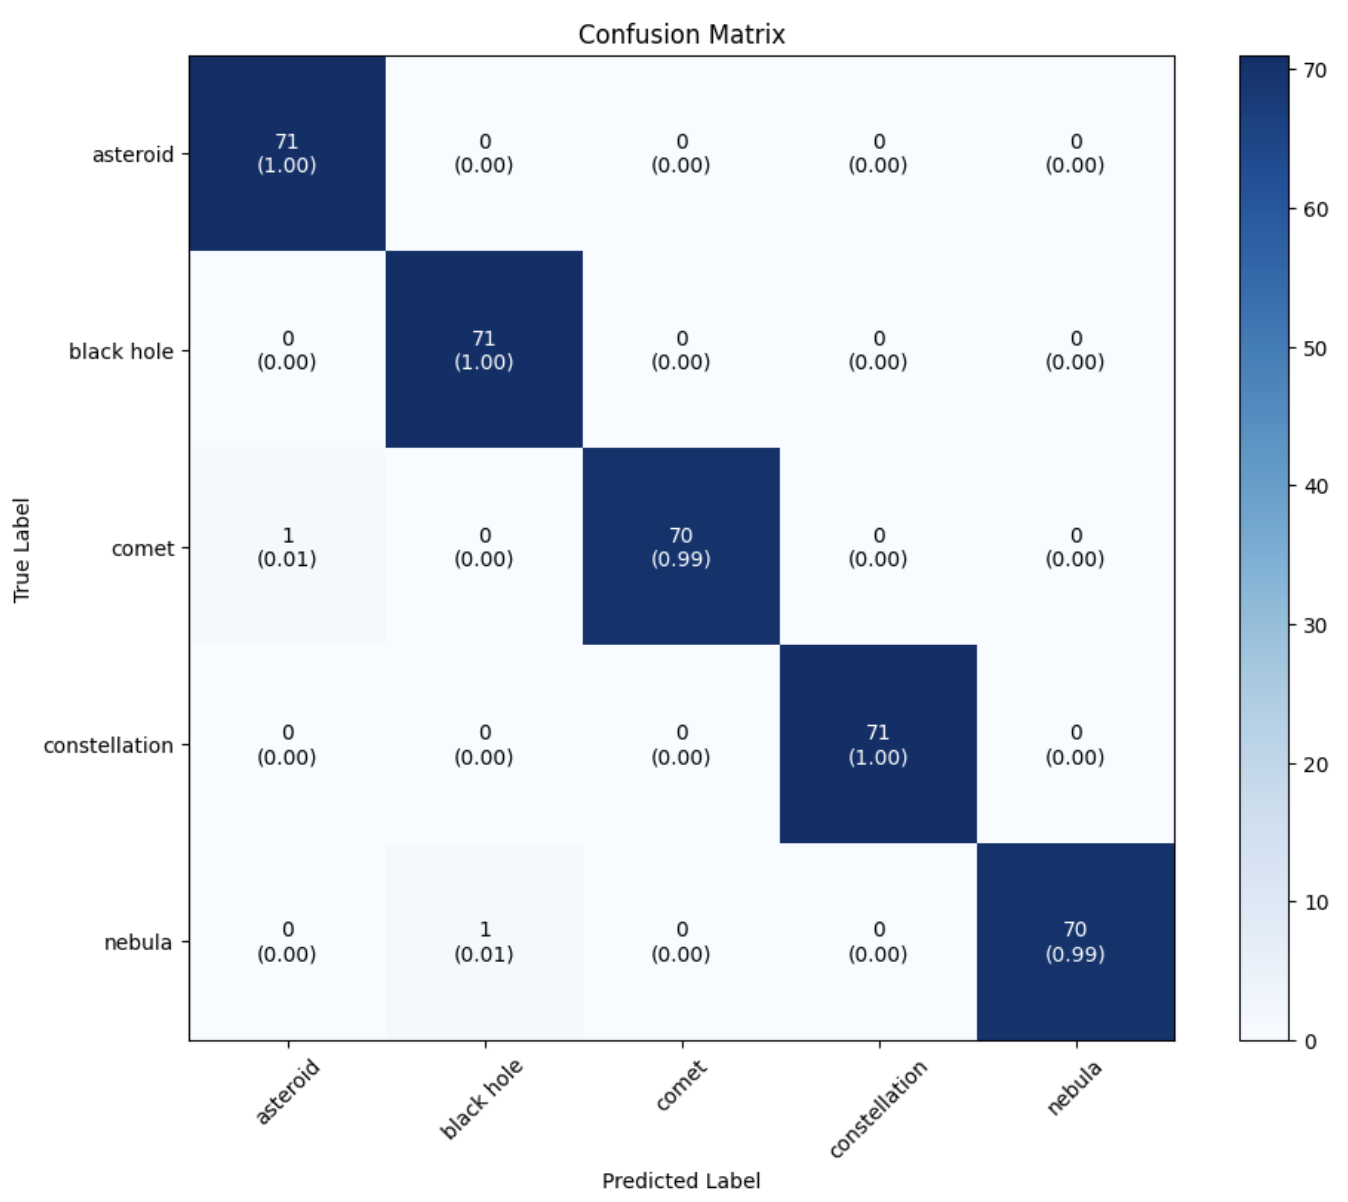
\includegraphics[width=\linewidth]{generated/Balance-CNN.png}
  {\footnotesize (a) CNN — Balanced\par}
\end{minipage}\hfill
\begin{minipage}{0.48\textwidth}
  \centering
  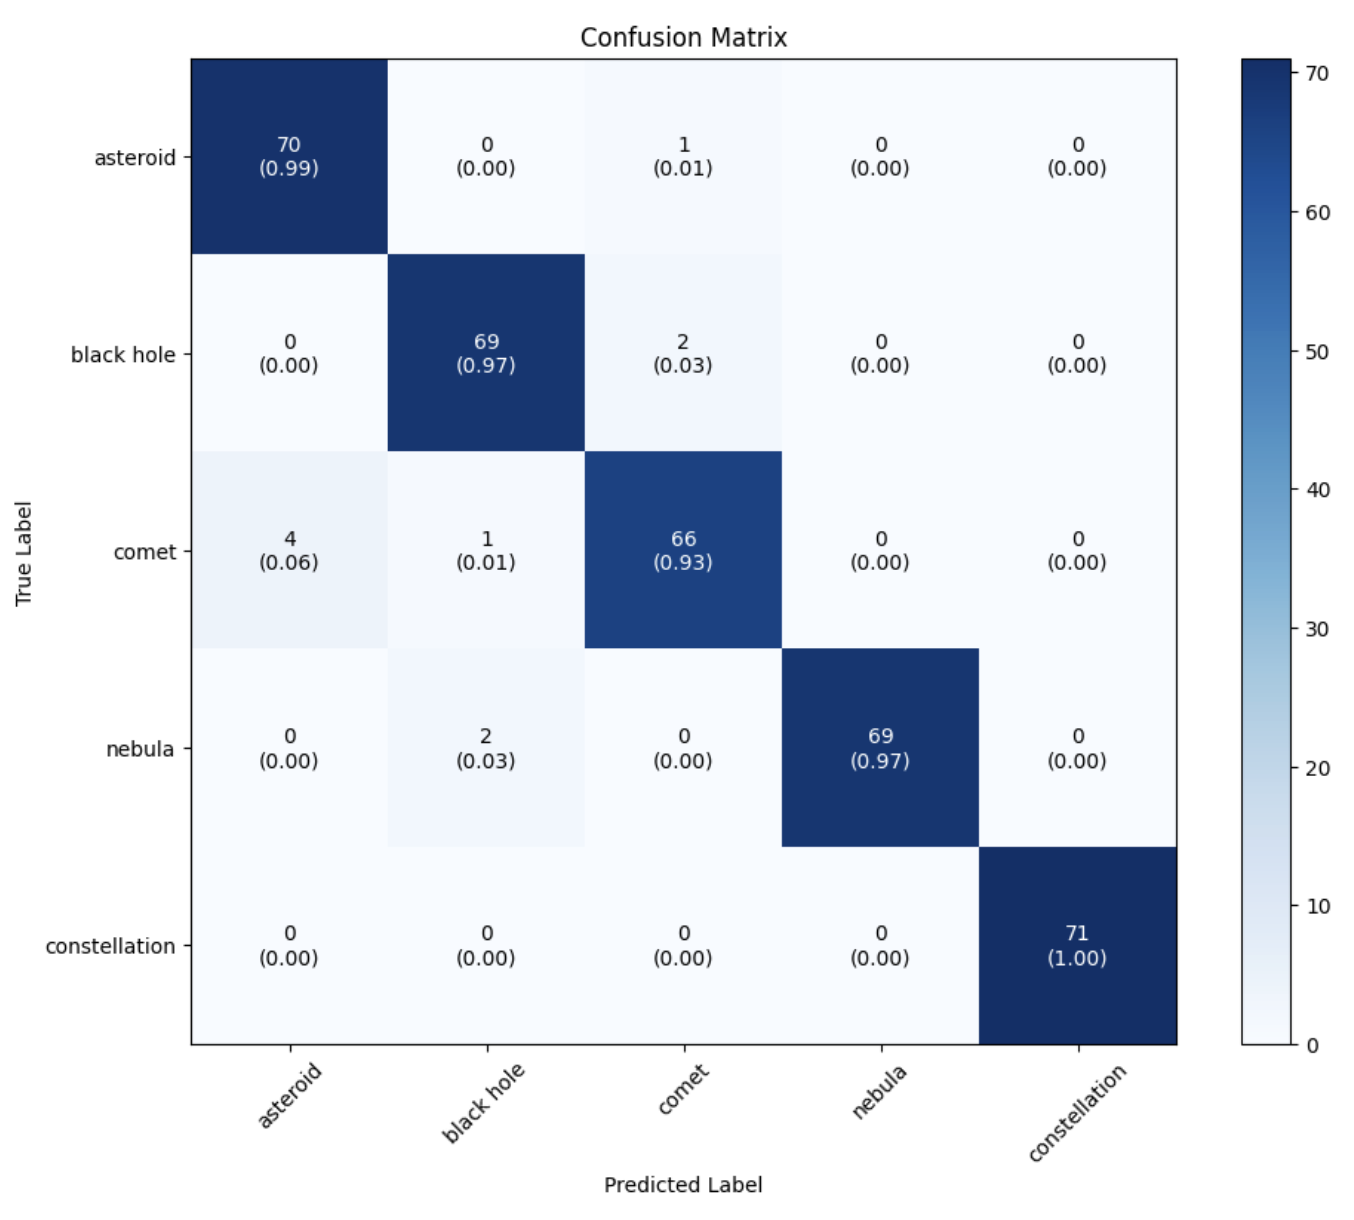
\includegraphics[width=\linewidth]{generated/Balance-VIT.png}
  {\footnotesize (b) ViT — Balanced\par}
\end{minipage}

\vspace{0.6em}

% Row 2 (Imbalanced)
\begin{minipage}{0.48\textwidth}
  \centering
  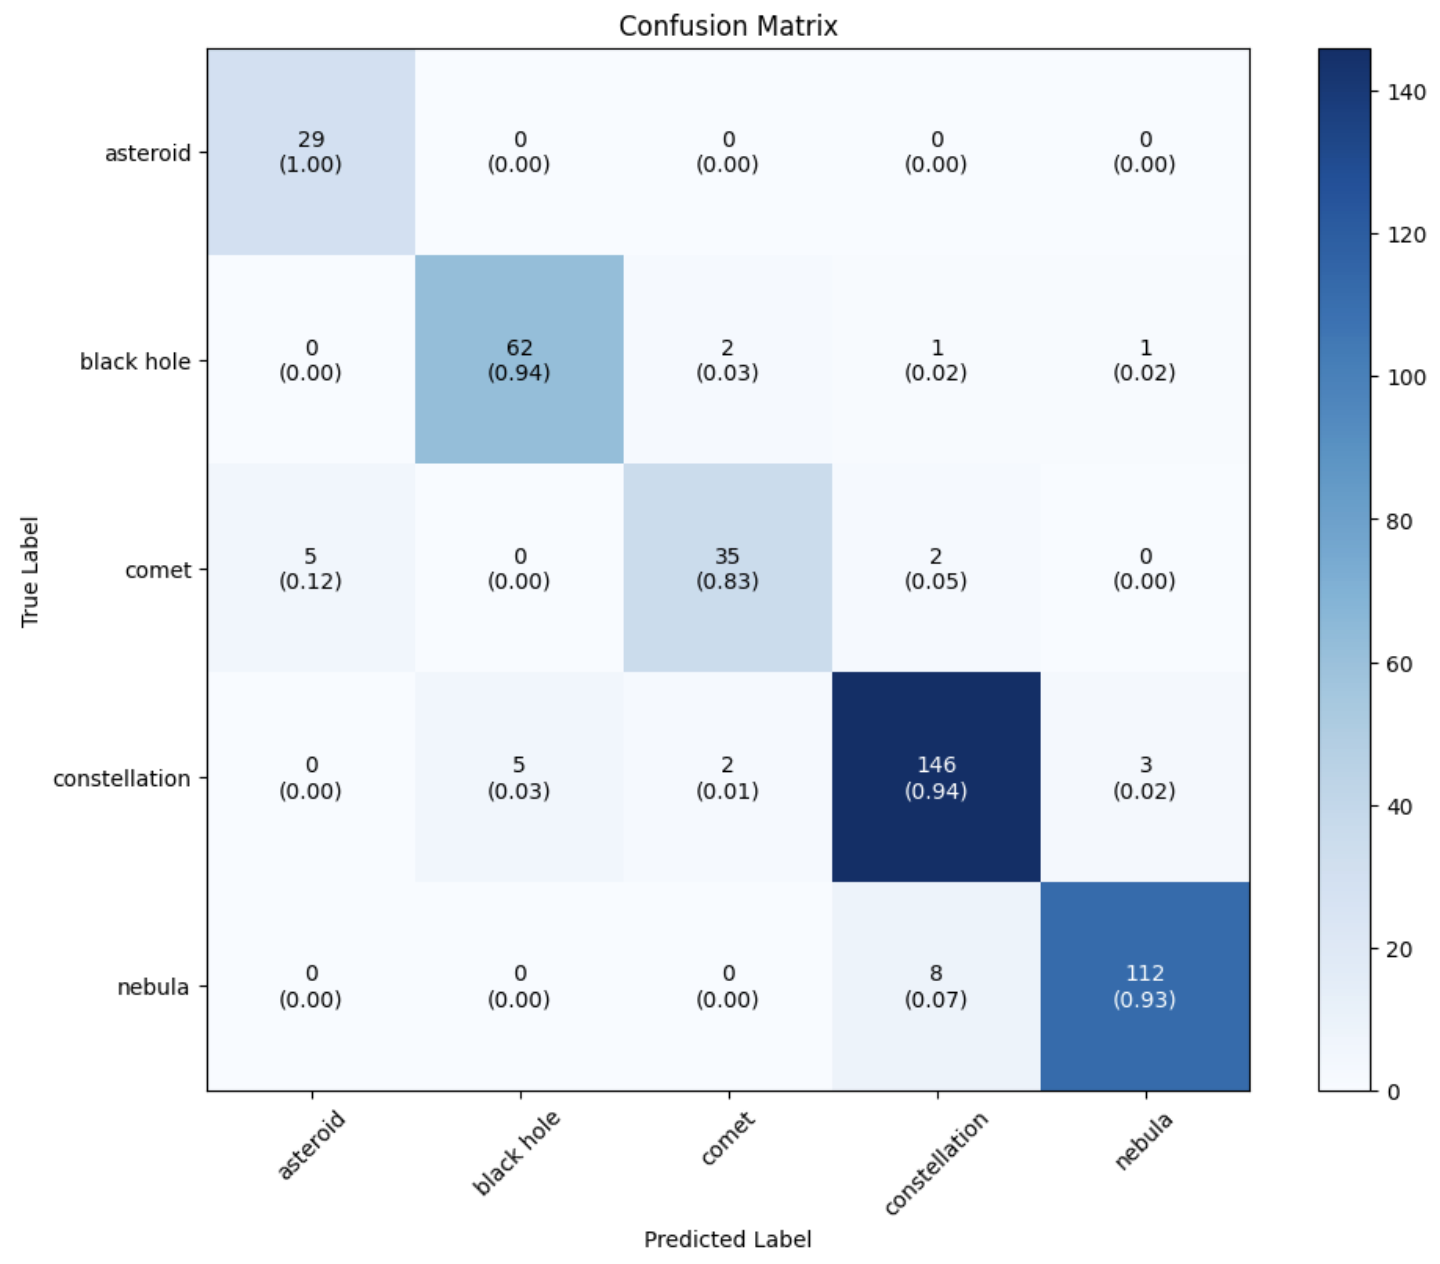
\includegraphics[width=\linewidth]{generated/Imbalance-CNN.png}
  {\footnotesize (c) CNN — Imbalanced\par}
\end{minipage}\hfill
\begin{minipage}{0.48\textwidth}
  \centering
  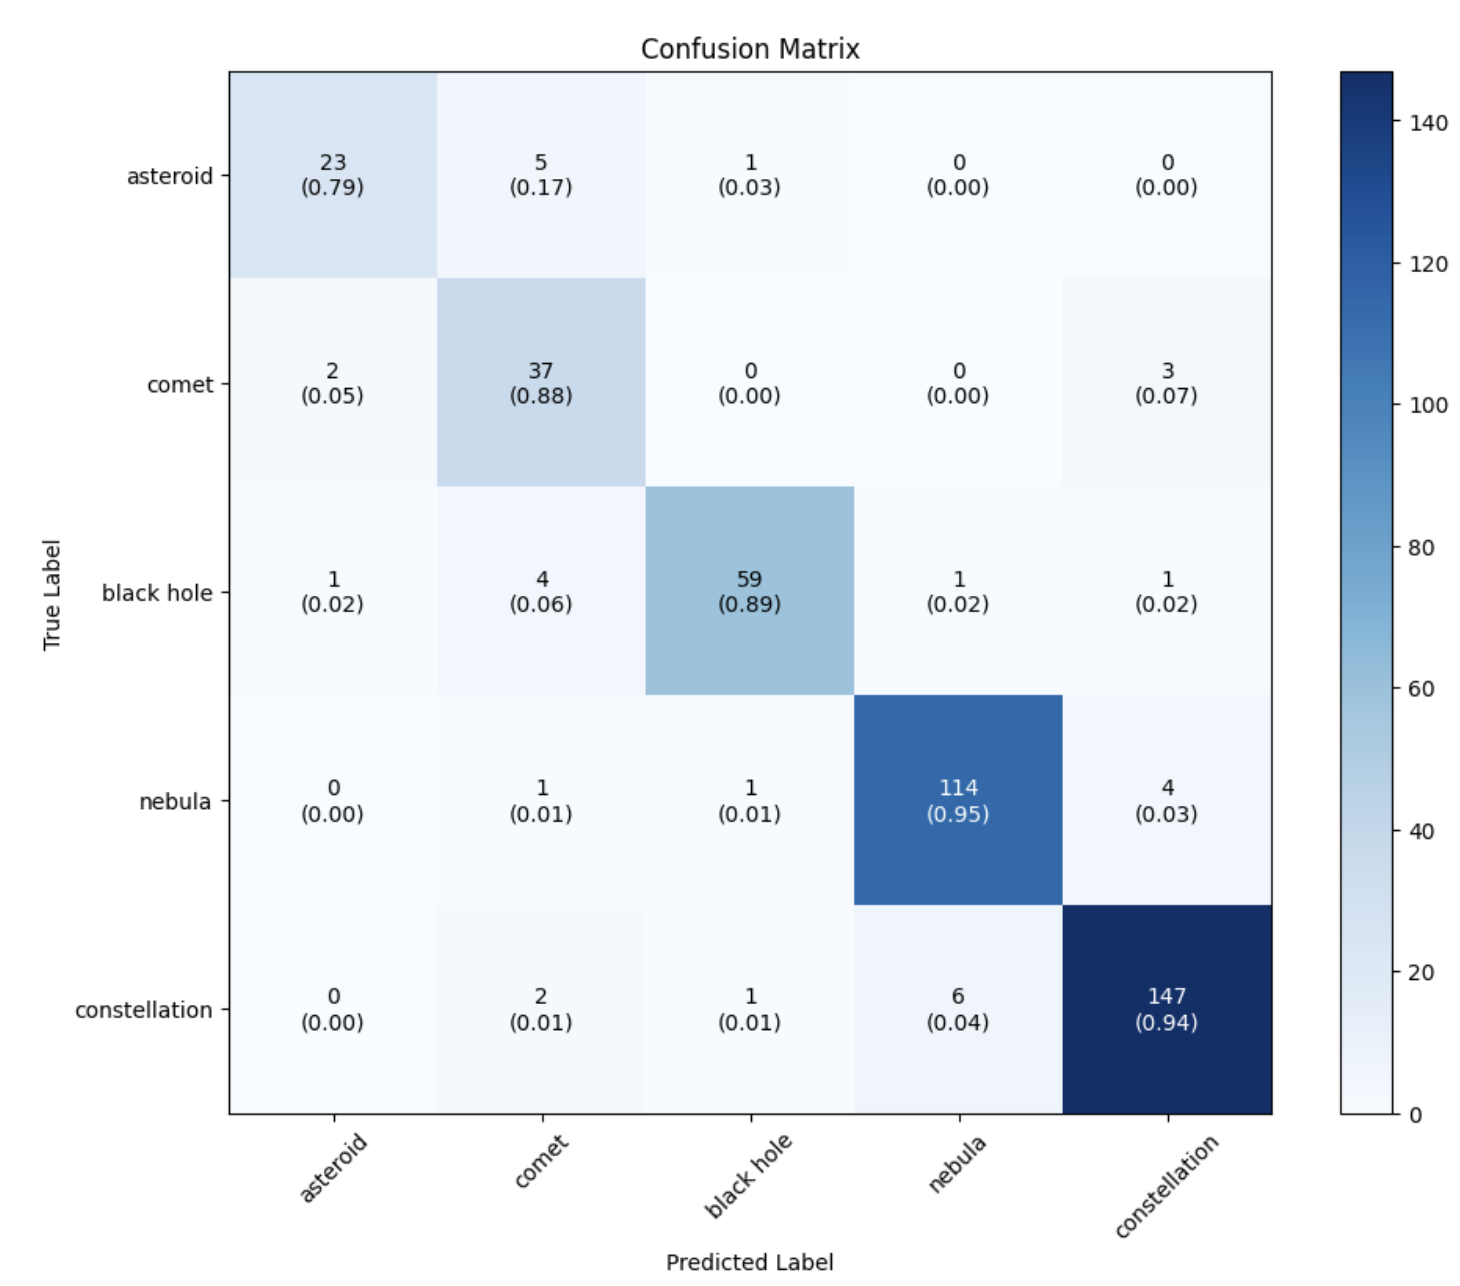
\includegraphics[width=\linewidth]{generated/Imbalance-VIT.png}
  {\footnotesize (d) ViT — Imbalanced\par}
\end{minipage}

\caption{Confusion matrices across regimes for EfficientNetB0 (CNN) and ViT-Base.}
\label{fig:cm-grid}
\end{figure*}

\FloatBarrier


\paragraph{Provenance.}
Both the imbalanced and balanced directories are deterministic \textbf{70:20:10} splits
derived from the original SpaceNet dataset~\cite{SpaceNetKaggle}.
We do not redistribute images; we share only file lists (manifests) that reference the
original files. Exact manifests for train/val/test (both splits) and all training logs
are included with our Kaggle notebooks and supplementary material.

\noindent\textbf{Efficiency.} Dataset inference time (s): EffB0 (51.97), ViT-Base (68.07), ViT-Small (68.34), ViT-Tiny (64.37). Model sizes as above. Training time per epoch (s): 198.9 / 637.3 / 651.0 / 571.3.

\subsection{Learning Curves (example: EffB0, 20 epochs)}
We observed rapid convergence with unstable early validation, then consistent gains.

\subsection{Ablations}
\textbf{4-class subset (no constellation).} Early 20-epoch runs exhibited lower test accuracy in some settings; later training and improved preprocessing closed the gap (details in notebooks). \\
\textbf{Loss variants.} Class-weighted CE consistently improved minority recall; focal loss ($\gamma{=}2$) provided marginal additional gains.



\section{Discussion}
\textbf{Accuracy vs Efficiency.} On balanced data, ViT variants approach CNN accuracy, but CNNs remain faster and smaller. On imbalanced data, EfficientNet edges ViT-Base in macro-F1 at lower cost. \\
\textbf{When to pick ViT.} Literature suggests ViTs can be more robust to noise and OOD and generalize across forgery types; if robustness trumps latency, ViTs (or CNN+ViT hybrids) are attractive.
\textbf{When to pick CNN.} For latency-constrained deployments or severe skew without heavy rebalancing, models like EfficientNetB0 provide strong baselines with small footprints.
Consistent with prior scaling results~\cite{Dosovitskiy2020ViT}, we expect ViTs to increasingly outperform small CNNs as data volume and/or pretraining scale grows; on SpaceNet’s modest size, EfficientNetB0 retains an efficiency edge while achieving competitive accuracy.
On balanced data, ViT-Base approaches CNN accuracy, but the CNN remains faster and smaller.

\section{Limitations}
Single dataset at 224\(\times\)224; additional astronomy corpora and higher resolutions left for future work. Some literature references are placeholders—add full bibliographic entries. Confusion matrices and per-class breakdowns are available in notebooks; include them as figures in a camera-ready version.

\section{Conclusion}
Using one dataset under two regimes, we showed how label distribution and architecture interact: balancing boosts all models; under skew, class-weighted CNNs are a safe default, while ViTs remain competitive at higher compute. Cross-domain evidence indicates ViTs may offer robustness advantages important for safety-critical applications.

\section*{Reproducibility}
Data: SpaceNet (Kaggle)\cite{SpaceNetKaggle}. 
Notebooks: \textbf{Imbalanced} (CNN and ViT-Base, 40 epochs)\cite{Gothi_ImbalCNN40_2025,Gothi_ImbalViTBase40_2025}; 
\textbf{Balanced} (CNN and ViT-Base, 40 epochs)\cite{Gothi_BalEfficientNet40_2025,Gothi_BalViTBase40_2025}. 

\bibliographystyle{IEEEtran}
\bibliography{references}

\end{document}
